\block{3. Creation of the dataset} {
        
    \begin{minipage}[t]{0.48\linewidth}

        \vspace{0.5cm}

        \textbf{\underline{Nanoalloys dataset}}

        \vspace{0.5cm}

        The final snapshots of the MD simulations are extracted, analyzed in terms of structure, and used to generate synthetic HRTEM images.
        
        \vspace{0.25cm}

        \begin{itemize}
            \item \textbf{Number of data:} 48000 simulated nanoalloy particles ;
            
            \vspace{0.25cm}
            
            \item \textbf{Large diversity of data} thanks to the random parameters of the MD simulations.
        \end{itemize}

        \vspace{1.2cm}

        \begin{center}
            \begin{tikzpicture}
                \node[anchor=west, inner sep=0] (image1) at (0,0) {
                    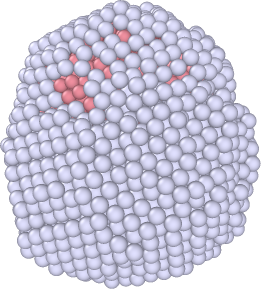
\includegraphics[width=0.11\linewidth]{Figure/particle_exemple.png}
                };

                \node[anchor=west, inner sep=0, xshift=0.15\linewidth] (image2) at (0,0) {
                    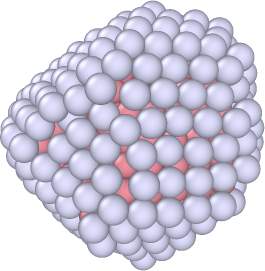
\includegraphics[width=0.11\linewidth]{Figure/particle_exemple2.png}
                };

                \node[anchor=west, inner sep=0, xshift=0.30\linewidth] (image3) at (0,0) {
                    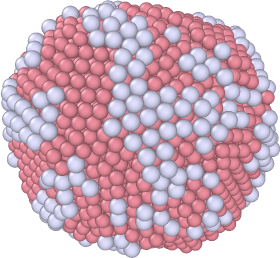
\includegraphics[width=0.11\linewidth]{Figure/particle_exemple3.png}
                };

                \node[anchor=west, inner sep=0, xshift=0.45\linewidth] (image4) at (0,0) {
                    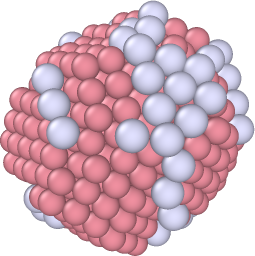
\includegraphics[width=0.11\linewidth]{Figure/particle_exemple4.png}
                };
            
                \node[anchor=north, align=center, yshift=-0.025\linewidth] at (current bounding box.south) {\small{Examples of the dataset}};
            \end{tikzpicture}
        \end{center}

        \vspace{1.2cm}

        \textbf{\underline{HRTEM images dataset}}

        \vspace{0.5cm}

        The \textbf{dataset of HRTEM images} is generated using \textbf{DrProbe}~[2] to simulate the HRTEM images associated with the nanoalloy dataset.
        
        \vspace{1.4cm}

        \begin{center}
            \begin{tikzpicture}
                \node[anchor=west, inner sep=0] (image1) at (0,0) {
                    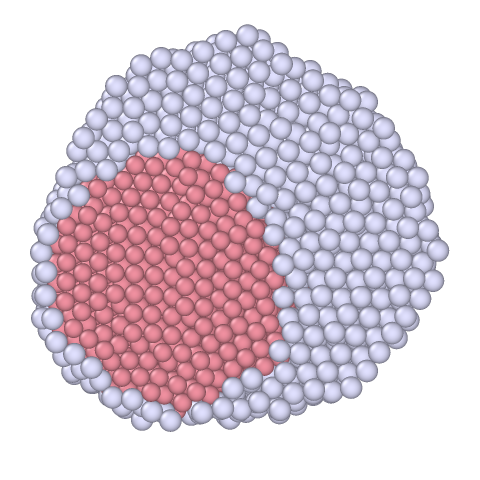
\includegraphics[width=0.22\linewidth]{Figure/md_to_hrtem.png}
                };

                \node[anchor=west, inner sep=0, xshift=0.38\linewidth] (image2) at (0,0) {
                    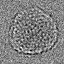
\includegraphics[width=0.18\linewidth]{Figure/hrtem.jpg}
                };

                \node[anchor=north, align=center] at (image1.south) {\small{Sample}};
                \node[anchor=north, align=center] at (image2.south) {\small{HRTEM image}};

                \draw[-{Latex[length=8mm,width=6mm]}, line width=1.4pt] ([xshift=0.05cm]image1.east) -- ([xshift=-0.20cm]image2.west);
                \node[anchor=south, align=center, font=\small] at ([yshift=0.1cm]$(image1.east)!0.5!(image2.west)$) {\textbf{DrProbe}};
            \end{tikzpicture}
        \end{center}
    \end{minipage}
    \hfill
    \begin{minipage}[t]{0.48\linewidth}
        
        \vspace{0.5cm}
        
        \textbf{\underline{Distribution of the core-shell index}}
        
        \vspace{0.5cm}
        
        The \textbf{core-shell index} $\eta$ is used to characterize the structure of the nanoalloys.
        
        \vspace{0.05cm}

        \begin{equation}
            \eta = 2\left| \frac{n^{out}_{Ag}}{n^{out}_{Ag} + n^{out}_{Co}} - \frac{n_{Ag}}{n_{tot}}\right| + 2\left| \frac{n^{in}_{Ag}}{n^{in}_{Ag} + n^{in}_{Co}} - \frac{n_{Ag}}{n_{tot}}\right| - \frac{d_{com}}{2r_{g}}
        \end{equation}
        
        \vspace{0.05cm}

        The first two terms measure how much the \textbf{\textcolor{colorAg}{Ag} concentration} in the \textbf{outer} and \textbf{inner} regions deviates from the overall composition of the particle.
        Here, $n^{out}_{Ag}$ and $n^{out}_{Co}$ denote the numbers of \textcolor{colorAg}{Ag} and \textcolor{colorCo}{Co} atoms in the \textbf{outer shell}, while $n^{in}_{Ag}$ and $n^{in}_{Co}$ refer to the \textbf{inner region}.
        The last term accounts for the distance $d_{com}$ between the centers of mass of the two species, normalized by the radius of gyration $r_g$.
        Taken together, these quantities can be used to quantify the degree of \textbf{core-shell} or \textbf{Janus} character of the nanoalloys, with larger $\eta$ values indicating a strong core-shell structure and smaller or negative values corresponding to a more mixed configuration.

        \vspace{0.4cm}

        \begin{center}
            \begin{tikzpicture}
                \node[anchor=center] (image) at (0,0) {
                    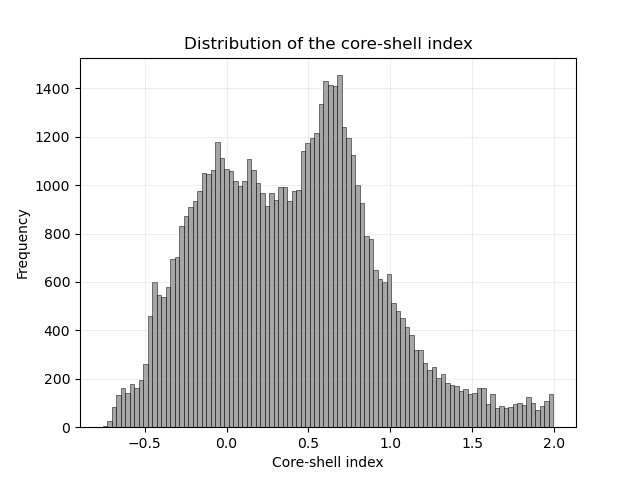
\includegraphics[width=0.55\linewidth]{Figure/distribution.png}
                };
            \end{tikzpicture}
        \end{center}
    \end{minipage}
}
